\section{Multi-Clustered Particle Filtering}

\begin{frame}
	\frametitle{Multi-Clustering Particle Filtering}
		\begin{columns}
			\column[T]{.5\textwidth}
			
			\begin{enumerate}
				\item<2-> system state evolution
				\item<3-> local system state estimation
				\item<4-> gathering global information
				\item<6-> clusterisation
				\item<7-> data association
				\item<8-> global estimation
			\end{enumerate}
			
			\column[T]{.5\textwidth}
			\centering
			\includegraphics[width=5.5cm]<1>{Figures/Mamot0.pdf}
			\includegraphics[width=5.5cm]<2>{Figures/Mamot1.pdf}
			\includegraphics[width=5.5cm]<3>{Figures/Mamot2.pdf}
			\includegraphics[width=5.5cm]<4>{Figures/Mamot3.pdf}
			\includegraphics[width=5.5cm]<5>{Figures/Mamot3Bis.pdf}
			\includegraphics[width=5.5cm]<6>{Figures/Mamot4.pdf}
			\includegraphics[width=5.5cm]<7>{Figures/Mamot5.pdf}
			\includegraphics[width=5.5cm]<8>{Figures/Mamot6.pdf}
		\end{columns}
\end{frame}

\begin{frame}
	\frametitle{Clustering Correlation}
	\begin{columns}[T]
		\column{.5\textwidth}
		\centering
		\begin{itemize}
			\item Particles' clusterisation in order to detect targets \\
				  $ \leadsto $ approximatively each cluster corresponds to an estimated target
			\item Dynamic threshold function used to separate the clusters
			\item It depends on:
			
			\begin{itemize}
				\item complexity of world
				\item expected number of targets
				\item field-of-view of agent's sensors
			\end{itemize}
		\end{itemize}
		
		\column{.6\textwidth}
		\centering
		
		\begin{tikzpicture}
			\node at (0,0) [draw=black,thick,inner sep=0pt]{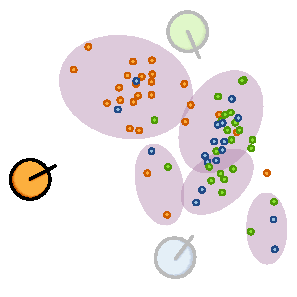
\includegraphics[width=2.5cm]{Figures/Mamot4.pdf}};
		\end{tikzpicture}
		\begin{tikzpicture}
			\node at (0,0) [draw=black,thick,inner sep=0pt]{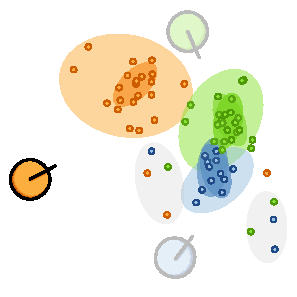
\includegraphics[width=2.5cm]{Figures/Mamot5.pdf}};
		\end{tikzpicture}\\
		\vspace{0.2cm}
		\begin{tikzpicture}
			\node at (0,0) [draw=black,thick,inner sep=0pt]{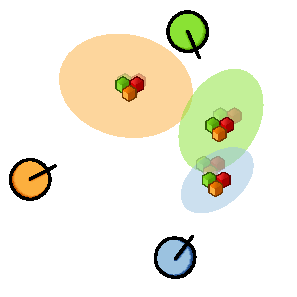
\includegraphics[width=3cm]{Figures/Mamot6.pdf}};
		\end{tikzpicture}
	\end{columns}
\end{frame}
